\documentclass[a4paper]{article}
\usepackage[utf8]{inputenc}
\usepackage[english]{babel}
\usepackage{amsmath,amsthm,amssymb}
\usepackage{geometry}
\usepackage{braket}
\usepackage{tikz}
\usepackage{placeins}

\newcommand{\HH}{\mathcal{H}}
\newcommand{\CC}{\mathbb{C}}
\DeclareMathOperator{\spn}{span}
\newcommand{\ppar}[1]{#1}
\newcommand{\pper}[1]{#1_{\perp}}
\newcommand{\norm}[1]{\left\lVert#1\right\rVert}


\title{Mangled Children \\ \large Quantum exploration of a classical epistemic
 puzzle}
\author{Krasimir Georgiev}

\begin{document}
\maketitle
\section*{Introduction} The muddy children puzzle is a well-known epistemic
puzzle that illustrates some features of the dynamics of knowledge. 
Quantum physics is normally perceived as a notoriously difficult to reason
discipline. It lacks connections with real world intuition and has bizarre
predictions. In this report we construct quantum analogues of the muddy
children puzzle. We explore these variants using a blend of quantum and
epistemic reasoning.

\section*{Muddy children} The  muddy children puzzle goes as follows: several
clever (logically omniscient) children are playing with mud; their father comes
and tells them (publicly announces): some of you have muddy faces.  Then he
proceeds to ask the same question over and over again: Do you know if you are
muddy? During each round of questioning, each child publicly announces its
answer truthfully at the same time. As a result, during first several rounds,
each child answers negatively. But at some specific round exactly the muddy
children answer positively. At first sight this is paradoxical: by listening to
the same answers of the same question over and over again, the children come to
learn new information.

For $n$ children, we may model the puzzle by an epistemic model where the worlds
are all the strings over $\{0, 1\}$ of length $n$, where $1$ at position $i$
denotes that the $i$-th child has mud on its face.  The indistinguishability
relation $R_i$ for the $i$-th child contains all the pairs of strings that
possibly differ only at the $i$-th position.  Suppose that $u \geq 1$ of the
children are actually muddy. The public announcement of the father effectively
deletes the world $0^n$. At round $r = 1, 2, \dots, u-1$, the public
announcements of the children delete all the worlds that contain $r$ ones. At
round $r = u$, since all worlds with a lower number of ones are deleted, all the
muddy children can distinguish the real world, so they give a positive answer.

\section*{Quantum world}

The postulates of quantum physics govern that the state space of a quantum
system corresponds to the one-dimensional (closed) subspaces of some Hilbert
space $\HH$ (over $\CC$). Quantum evolution is captured by unitary
transformations. The possible properties of a quantum system correspond to
subsets of the state space. The properties corresponding to the closed subspaces
of $\HH$ are called testable. Only testable properties of a quantum system can
be observed in principle~\cite{wlogqm}, which is in a sharp contrast with the classical case
where any property of a physical system can be observed in principle. This model
of the quantum world necessarily contains much more ``quantum information'' than
what is physically accessible. Many interesting properties of a quantum systems,
like being entangled, are not testable.

Quantum observations of testable properties have the peculiar property of
possibly probabilistically altering the real world state of a quantum system. As
such, quantum observations cannot be treated as a purely epistemic actions
extracting knowledge about the quantum system, but as a complex dynamic action
on the quantum system, having both epistemic and ontic side
effects~\cite{wlogqm}~\cite{dlpqb}.

The dynamics of quantum observations works as follows. Suppose the quantum
system is in a state $\spn s$ for some unit vector $s \in \HH$ and suppose we
perform a quantum observation of a testable property corresponding to the closed
subspace $P \subseteq \HH$. The vector $s$ is split in two components: the one
parallel to $P$ (or equivalently, belonging to $P$), and the one perpendicular
to it: $s = \ppar{P}(s) + \pper{P}(s)$ (we consistently apply this notation for
these two components throughout this report). Note that $\norm{\ppar{P}(s)}^2 +
\norm{\pper{P}(s)}^2 = 1$, since $s$ is a unit vector. With probability
$\norm{\ppar{P}(s)}^2$ the quantum test succeeds and the quantum system
collapses to the state $\spn \ppar{P}(s)$.  Similarly, with probability
$\norm{\pper{P}(s)}^2$ the quantum test fails and the quantum system collapses
to the state $\spn \pper{P}(s)$. Note that the probabilities here are
``external'' in a sense: the observation will definitely yield some answer,
after which the initial state of the system is lost. But if we had many
independent copies of the initial state and repeated the observation on them,
then the probabilities for the outcomes will be as described.

Essentially, a quantum observation forces the quantum system to
(probabilistically) collapse to the state that is most like the initial state
and is fully consistent with the result of the observation. This is reminiscent
of a public announcement followed by belief revision in an epistemic model.
Quantum observations are repeatable (idempotent): repeating the same observation
twice always yields the same result and the quantum state doesn't change after
the first observation. They are not monotonic however: typically a sequence of
distinct observations can move the quantum system through many different quantum
states.

\section*{Quantization}
We have to reconsider the building blocks of the muddy children puzzle in a
quantum setting. Let us think of the mud on the faces of the children as a
quantum system in some state that corresponds to the subspace $\spn{s}$ for some
unit vector $s \in \HH$. The act of looking at the children's faces becomes a
quantum observation.  It no longer makes much sense in general to consider
absolute statements like: ``you are muddy'', because the non-monotonicity of
quantum observations makes this statement quite unstable and too strong.
Instead, we will consider dynamic versions of this statement that have natural
quantum semantics. Suppose that the quantum observation of some face corresponds
to the subspace $M \subseteq \HH$. The following are possible quantum dynamic 
versions of the statement ``you are muddy'':

\begin{itemize}
\item \emph{Observing your face will possibly turn out muddy.}
    This corresponds to the condition $s \not\perp M$.
\item \emph{Observing your face will surely turn out muddy.}
    This corresponds to the condition $s \in M$.
\item \emph{Observing your face will turn out muddy with probability $P \in
    [0,1]$.} 
    This corresponds to the condition $\norm{\ppar{M}(s)}^2 = P$ and generalizes
    the previous versions.
\end{itemize}
Note that in a general state these statements are impractical for direct 
verification because of their external probabilistic nature.

We will assume further that the father is a quantum omniscient entity. As such,
he has direct access to the full quantum information about the real world
quantum state without disturbing it. So he plays the role of a god (or at least
as the one that prepared the quantum system) in the quantum versions of the
puzzle.

The next issue is quantum disjunction. We are concerned in interpreting the
initial announcement of the father: someone is muddy. Since the union of closed
subspaces is not necessarily a closed subspace, in general the classical version
of that statement does not correspond to an observable property of the system.
In general, quantum disjunction corresponds to the span of the classical
disjunction and captures the concept of superpositions~\cite{wlogqm}.
In the next section, we will analyze a version of the puzzle in which the
property \emph{after (joint) observation, it is impossible that everyone is
clean} happens to be a testable property. There is a weaker form of quantum
disjunction that is interpreted by the span of the interpretation of the
classical disjunction. We see a setting in which this quantum disjunction is too
weak to give the children any new information whatsoever. Note that there is no
such issue occurring with the conjunction of quantum properties, since the
intersection of closed subspaces is itself a closed subspace.

Another issue is with simultaneous observations. Since an observation has an
ontic effect, it is in general impossible for all observers to observe the
system at the same time. Only in specific cases (as in the next section)
simultaneous observations will make sense. When this might lead to problems, we
will number the children by $1, 2, \dots, n$ and assume (that it is public
knowledge) that they make their quantum observations in that order. Note that
this does not necessarily imply a restriction to their simultaneous classical
answer to the question of the father.

Finally, the question of the father needs to be adapted so that it blends the
quantum and epistemic features of the situation. We will consider variants of 
the following plausible adaptation:
\emph{After you did the quantum observation (that you were supposed to do,
    typically observing the others), do you know that if your face is observed,
it will (possibly/surely) be dirty?}

\section*{Compound quantum mud}
For our first concrete version of the puzzle, let us consider a situation in
which there are just $n = 2$ children: Alice and Bob. There is a qubit for the
mud on each one's face. The state space of this quantum system is the set of
one-dimensional subspaces of the four dimensional Hilbert space $\HH =
(\CC^2)^{\otimes 2}$
constructed from the tensor product of two two-dimensional identical Hilbert
spaces~\cite{lqp22} with an
orthonormal basis $\{\ket{ab}, \ket{aB}, \ket{Ab}, \ket{AB}\}$. Observing that
Alice's face is muddy corresponds to the subspace $\spn\{\ket{Ab},\ket{AB}\} =
\spn\ket{A}$\footnote{We may think about $\ket{A}$ either as an abuse of
notation, or~\cite{geomcs} we may make it a formal object by interpreting it as
a bivector (two-dimensional analogue of a vector) generated by the outer product
of two vectors in the Clifford algebra of subspaces of $\HH$.}.  Observing that
Alice's face is clean corresponds to the subspace $\spn\{\ket{ab},\ket{aB}\} =
\spn\ket{a}$. Similarly we can define the subspaces $\spn\{\ket{aB}, \ket{AB}\}
= \spn\ket{B}$ for muddy Bob and $\spn\{\ket{ab},\ket{Ab}\} = \spn\ket{b}$ for
clean Bob. A general state of this system has the form $\spn{s}$ for some unit
vector $s = \alpha\ket{ab} + \beta\ket{aB} + \gamma\ket{Ab} + \delta\ket{AB}$,
for some $\alpha, \beta, \gamma, \delta \in \CC$ such that $|\alpha|^2 +
|\beta|^2 + |\gamma|^2 + |\delta|^2 = 1$.  Assume that all of this is common
knowledge, so our initial epistemic model contains all of these $s$ and the
indistinguishability relations $R_i$ are the full relations over the state
space.

Now the father comes and tells them: \emph{it is impossible that after an
observation of both of you, both of you are clean}. Note that this is a yet
another variant of the initial announcement that can be formulated in this
particular setting. It is true iff $\alpha = 0$. The public announcement of this
statement effectively deletes the states having $\alpha \neq 0$ from the
epistemic model, leaving us with a general state of the epistemic model of the
form $s = \beta\ket{aB} + \gamma\ket{Ab} + \delta\ket{AB}$.

Now the father asks the children if they know that they are dirty, or more
precisely, if \emph{after having observed the other child's face, they came to 
know that observing their own face will surely turn out muddy}. Firstly Alice
observes Bob's face and by doing so, she collapses the system to a state that is
consistent with her observation. In detail:
\begin{enumerate}
\item She might observe that Bob is muddy (which happens with probability
    $|\beta|^2 + |\delta|^2$). In this case the system collapses to the state
    $\spn s'$ for the unit vector $s' = \frac{\beta\ket{aB} +
    \delta\ket{AB}}{\sqrt{|\beta|^2 + |\delta|^2}}$. Since this new state has a
    nonzero projection along both $\ket{a}$ and $\ket{A}$, she answers ``no'' to
    the father's question.

\item She might observe that Bob is clean (which happens with probability
    $|\gamma|^2$). In this case the system collapses to the state $\spn{s''}$
    for the unit vector $s'' = \frac{\gamma\ket{Ab}}{|\gamma|}$. Since $s'' \in
    \spn\ket{A}$, she answers ``yes'' to the father's question (and more
    precisely, she knows that observing her face will surely turn out to be
    muddy).
\end{enumerate}

Now comes Bob's turn. Since he is logically omniscient, he will deduce the
previous argument by himself. Note that at the time of his quantum observation
of Alice's face, Alice hasn't announced her answer yet. What might happen is:
\begin{enumerate}
\item He might observe that Alice is clean. Then it cannot be the case that the
    system was in state $\spn s''$ right before that observation, because $s''
    \perp \ket{a}$. Thus the system must have been at state $s'$.  But since $s'
    \in \spn \ket{B}$, Bob deduces that observing his face will surely turn out
    to be muddy and answers `yes'' to the father's question.

\item He might observe that Alice is dirty. This is possible from both the
    states $\spn s'$ and $\spn s''$, and the observation collapses them to the
    states $\spn\ket{AB}$ and $\spn\ket{Ab}$, respectively. Since observing
    Bob's face from these two states will surely yield the two distinct
    outcomes, he answers `no'' to the father's question.
\end{enumerate}

Now they both publicly announce their answers. If it is not the case that both
of them end up muddy after the first round, exactly the muddy one will
answer ``yes''. If both of them are muddy, both of them will answer ``no'', and
the system will collapse to the pure state $\spn\ket{AB}$. Since the children
will deduce this, at the next round the kids will not even need to perform any
new quantum observations to know that they are definitely (and regardless of new
observations) both muddy.

The striking thing is that in this setting \emph{the (dynamic epistemic) 
situation turns out to be no different than the classical one}: at some
round exactly the muddy children (at that time) announce that they know they're
muddy. This is also true in the general case: essentially for $n$ children, after
the first two children observe the others, the quantum state (probabilistically) 
collapses to a pure (essentially classical) state that is consistent with the
first two quantum observations. So, there are no bizarre quantum effects to
observe in this version of the puzzle. The reason for this seems to
be the combination of two constraints to the quantum system: \emph{mutual
orthogonality between all observable states} and \emph{no quantum evolution}.
This ensures that such a system is actually monotone with respect to the
repetitions of observations. This has the epistemic effect of forming a kind of
classical, epistemic superposition of possible worlds that exactly corresponds
to the logically possible worlds based on the knowledge so far. This case is
reminiscent of the definition of a Classical Epistemic Frame from~\cite{corrkn},
where all states are fully separable.

\section*{Quantum sharing of mud}
In this version, we restrict the quantum state space of the mud $\HH$ to be a
two-dimensional Hilbert space instead of a four-dimensional one. Here the
observations of the faces of Alice and Bob correspond to two different
orthonormal basis of $\HH$. We will consider a version where these two basis are
\emph{as distinct as possible} in a sense. Namely, suppose that the two unit
vectors $\ket{0}$ and $\ket{1}$ form an orthonormal basis of $\HH$ and let they
correspond to the possible outcomes of observing Alice's face: $\ket{a} =
\ket{0}$ and $\ket{A} = \ket{1}$. Take Bob's basis to be: $\ket{b} = \ket{-} =
\frac{\ket{0} - \ket{1}}{\sqrt{2}}$ and $\ket{B} = \ket{+} = \frac{\ket{0} +
\ket{1}}{\sqrt{2}}$ (see Figure~\ref{fig:shab})\footnote{Incidentally, this
gives us an interesting quantum religious possibility that God created Eve as a
unitary transformation of Adam (which, as opposed to the classical case,
automatically works in the opposite direction).}.
\begin{figure}
    \centering
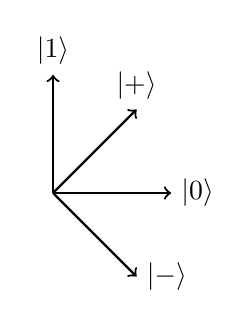
\begin{tikzpicture}[scale=1.5]
    \draw[->,thick] (0,0) -- (0,1) node [above] {$\ket{1}$};
    \draw[->,thick] (0,0) -- (1,0) node [right] {$\ket{0}$};
    \draw[->,thick] (0,0) -- (0.707,0.707) node [above] {$\ket{+}$};
    \draw[->,thick] (0,0) -- (0.707,-0.707) node [right] {$\ket{-}$};
\end{tikzpicture}
    \caption{Relative position of the basis in the quantum sharing version}
    \label{fig:shab}
\end{figure}
Assume that this is common knowledge, so initially the general state of the
system is $\spn s$ for some unit vector $s = \alpha \ket{0} + \beta \ket{1},
|\alpha|^2 + |\beta|^2 = 1$.  Let us consider the initial announcement of the
father. Note that now \emph{observing both faces is impossible.} This is an
instance of Heisenberg's uncertainty principle and is due to the fact that the
two observations do not correspond to orthogonal subspaces. So we cannot use the
interpretation from the previous version here.  Suppose the father's
announcement is: \emph{observing Alice's face will possibly turn out muddy,
(classical) or, observing Bob's face will possibly turn out muddy.} This
corresponds to the condition $\beta \neq 0$ (classical) or $\alpha + \beta \neq
0$. But if $\beta = 0$, then $\alpha + \beta \neq 0$ since $s$ is a unit vector.
So \emph{father's initial announcement is true at every possible quantum world
    and has no epistemic (in terms of deletion of possible worlds) effect
whatsoever.} Note that since quantum disjunction is weaker than classical
disjunction, the same will be true if we assumed that the father initially
announces using quantum disjunction instead of a classical one.

First Alice observes Bob's face. That has the effect of probabilistically
collapsing the system into the state $\spn s'$ for $s' \in \{\ket{-},\ket{+}\}$.
In any of these two states, if Alice's face is observed which corresponds to
collapsing along the $\{\ket{0},\ket{1}\}$ basis, has an equal probability $P =
\frac{1}{2}$ for both possible outcomes.  Thus, Alice doesn't know (surely) if
she would become muddy after observation or not. But she knows that
\emph{observing her face will turn out muddy with probability $\frac{1}{2}$.}
The situation for Bob is symmetric: after observing Alice's face, he knows that
he might turn out muddy with probability exactly $\frac{1}{2}$. An interesting
effect is that he knows that before observing Alice's face, he was either
definitely clean or definitely dirty (since $s' \in \{\ket{-}, \ket{+}\}$), but
\emph{the act of observing her face completely destroys the certainty of his own
face}.  Now that is an example of a truly quantum effect. We see that this
process will proceed indefinitely: it will always be the case that observing one
of the children will totally mess up the other's face.

We have seen how observing along non-orthogonal subspaces may lead to
non-classical behaviours. But what about quantum evolution? Well, since the two
distinct basis of the quantum system are connected by a unitary transformation
(rotation by $\frac{\pi}{4}$), we may simulate it by a situation in which we
only allow measurement along the $\{\ket{0},\ket{1}\}$ basis, but allowing each
child to apply the correct unitary transformation (rotation by $\frac{\pi}{4}$
in the right direction) before performing the observation along
$\{\ket{0},\ket{1}\}$.

\section*{Electron spin mud}
In particle physics, the spin of the electron is an interesting quantum system.
It can be observed along the three spacial directions $X, Y$ and $Z$ and the
observation yields a binary outcome $+$ or $-$. Consider a version of the puzzle
with three children, XBob, YChris and ZAlice. The mud in this case is the spin
of an electron and the three children's faces correspond to the three spacial
dimensions. Physics governs that the state space of the electron mud coincides
with the one from the previous version: a two-dimensional Hilbert space $\HH$.
The basis for ZAlice and XBob in this situation are the same as the basis for
Alice and Bob in the previous: $\{\ket{0},\ket{1}\}$ and $\{\ket{-},\ket{+}\}$,
respectively. The additional component of the puzzle is the basis for YChris,
which is $\ket{y_+} = \frac{\ket{0}+i\ket{1}}{\sqrt{2}}$ in case he is muddy and
$\ket{y_-} = \frac{\ket{0}-i\ket{1}}{\sqrt{2}}$ in case he is clean. The initial
announcement of the father here would be even weaker than in the previous
version, thus will not have any epistemic effect. Note that ZAlice cannot
observe both XBob's and YChris's faces, since their basis are not mutually
orthogonal. Suppose ZAlice observes XBob's face. The analysis of this proceeds
in the same way as in the previous version and after the observation the system
collapses to a state $\spn s'$ for some $s' \in \{\ket{-},\ket{+}\}$ (which only
Alice knows). Also she knows that after the observation her face becomes
completely uncertain (because $|\braket{0|s'}|^2 = |\braket{1|s'}|^2 =
\frac{1}{2}$). Let us analyze what effect on YChris's face has Alice's
observation of Bob's face. If $s' = \ket{+}$, since 
$\braket{+|y_+} = \frac{1}{2}(\bra{0} + \bra{1})(\ket{0} + i\ket{1}) =
\frac{1+i}{2}$, the probability of observing a muddy YChris becomes
$\frac{1}{4}(1+i)(1-i) = \frac{1}{2}$. Similarly, if $s' = \ket{-}$, since
$\braket{-|y_+} = \frac{1}{2}(\bra{0} - \bra{1})(\ket{0} + i\ket{1}) =
\frac{1-i}{2}$, the probability of observing a muddy YChris is still
$\frac{1}{2}$. Similarly we can see that the same happens in general:
\emph{observing any child makes the other two's faces completely uncertain.}
We may see this again as an instance of the uncertainty principle.

\begin{thebibliography}{9}
\bibitem{corrkn}
A. Baltag, S. Smets. ``Correlated Knowledge, An Epistemic-Logic View on 
Quantum Entanglement'', International Journal of Theoretical Physics

\bibitem{wlogqm}
A. Baltag, S. Smets. ``What can Logic Learn from Quantum Mechanics?'',
presented at the ECAP 2005 workshop on quantum information in Lisbon,
Portugal, 2005

\bibitem{lqp22}
A. Baltag, S. Smets. ``LQP: The Dynamic Logic of Quantum Information'', section
2.2. 
Mathematical Structures in Computer Science, 16 (3): 491-525, 2006. 
Cambridge University Press.

\bibitem{dlpqb}
A. Baltag, S. Smets. ``A Dynamic - Logical Perspective on Quantum Behavior'', 
in I. Douven and L. Horsten (eds.) Studia Logica , special issue on Applied Logic in the Philosophy of Science, vol 89, pp.185-209, 2008.

\bibitem{geomcs}
L. Dorst, D. Fontijne; S. Mann. ``Geometric algebra for computer science: an 
object-oriented approach to geometry'', Amsterdam: Elsevier/Morgan Kaufmann
\end{thebibliography}

\end{document}
